\documentclass{article}
% !TEX encoding = UTF-8 Unicode
% !TEX root = docs/source/main.tex

\usepackage{titlesec}
\usepackage{tcolorbox}
\usepackage[margin=1in]{geometry}
\usepackage{float}
\usepackage{graphicx}
\usepackage[export]{adjustbox}


\titleformat*{\section}{\huge\bfseries}
\titleformat*{\subsection}{\LARGE\bfseries}
\titleformat*{\subsubsection}{\large\bfseries}
\titleformat*{\paragraph}{\large\bfseries}
\titleformat*{\subparagraph}{\small\bfseries}
\newcommand{\myparagraph}[1]{\paragraph{#1}\mbox{}\\}


\usepackage{listings}


\definecolor{CPPLight}  {HTML} {686868}
\definecolor{CPPSteel}  {HTML} {888888}
\definecolor{CPPDark}   {HTML} {262626}
\definecolor{CPPBlue}   {HTML} {4172A3}
\definecolor{CPPGreen}  {HTML} {487818}
\definecolor{CPPBrown}  {HTML} {A07040}
\definecolor{CPPRed}    {HTML} {AD4D3A}
\definecolor{CPPViolet} {HTML} {7040A0}
\definecolor{CPPGray}  {HTML} {B8B8B8}
\definecolor{backcolour}{rgb}{0.95,0.95,0.92}

\tcbset{colback=white,colframe=black!10}

\lstset{
    columns=fixed,       
    numbers=none,                                        
    frame=none,                                          
    backgroundcolor=\color{backcolour},            
    keywordstyle=\color[RGB]{255,0,127},                 
    numberstyle=\footnotesize\color{darkgray},
    commentstyle=\it\color[RGB]{0,153,76},                
    stringstyle=\rmfamily\slshape\color[RGB]{128,0,0},   
    showstringspaces=false,  
    basicstyle=\ttfamily\footnotesize,                     
    language=SQL,                                        
    morekeywords={},
    emphstyle=\color{CPPViolet}, 
}

\title{Documentazione di progetto}
\author{Nicola Panizzolo, Tommaso Soncin, Michael Sarto}
\date{CT006 2023/2024}
\usepackage{tgadventor}

%\setcounter{section}{-1}
\begin{document}

\lstset{inputencoding = utf8,  % Input encoding
    extendedchars = true,  % Extended ASCII
    literate      =        % Support additional characters
      {á}{{\'a}}1  {é}{{\'e}}1  {í}{{\'i}}1 {ó}{{\'o}}1  {ú}{{\'u}}1
      {Á}{{\'A}}1  {É}{{\'E}}1  {Í}{{\'I}}1 {Ó}{{\'O}}1  {Ú}{{\'U}}1
      {à}{{\`a}}1  {è}{{\`e}}1  {ì}{{\`i}}1 {ò}{{\`o}}1  {ù}{{\`u}}1
      {À}{{\`A}}1  {È}{{\'E}}1  {Ì}{{\`I}}1 {Ò}{{\`O}}1  {Ù}{{\`U}}1
      {ä}{{\"a}}1  {ë}{{\"e}}1  {ï}{{\"i}}1 {ö}{{\"o}}1  {ü}{{\"u}}1
      {Ä}{{\"A}}1  {Ë}{{\"E}}1  {Ï}{{\"I}}1 {Ö}{{\"O}}1  {Ü}{{\"U}}1
      {â}{{\^a}}1  {ê}{{\^e}}1  {î}{{\^i}}1 {ô}{{\^o}}1  {û}{{\^u}}1
      {Â}{{\^A}}1  {Ê}{{\^E}}1  {Î}{{\^I}}1 {Ô}{{\^O}}1  {Û}{{\^U}}1
      {œ}{{\oe}}1  {Œ}{{\OE}}1  {æ}{{\ae}}1 {Æ}{{\AE}}1  {ß}{{\ss}}1
      {ç}{{\c c}}1 {Ç}{{\c C}}1 {ø}{{\o}}1  {Ø}{{\O}}1   {å}{{\r a}}1
      {Å}{{\r A}}1 {ã}{{\~a}}1  {õ}{{\~o}}1 {Ã}{{\~A}}1  {Õ}{{\~O}}1
      {ñ}{{\~n}}1  {Ñ}{{\~N}}1  {¿}{{?`}}1  {¡}{{!`}}1
      {°}{{\textdegree}}1 {º}{{\textordmasculine}}1 {ª}{{\textordfeminine}}1
  }

\maketitle
\tableofcontents
\newpage

\section{Introduzione}
\subsection{Tema del progetto}
\par
Viene richiesto di curare il design e l'implementazione di una web application per la valutazione interna dei
progetti di ricerca da sottoporre per finanziamento all'Unione Europea. I ricercatori devono poter creare
nuovi progetti da sottoporre a valutazione, ciascuno dei quali comprende una descrizione testuale ed uno o
pi`u documenti in formato PDF da valutare, possibilmente di tipo diverso (data management plan, ethics
deliverable, ecc.). Ciascun progetto ha uno stato, fra cui:
\begin{itemize}
    \item approvato: i valutatori hanno espresso parere favorevole e non sono più possibili modifiche;
    \item sottomesso per valutazione: sottoposto per la prossima finestra di valutazione, ma non ancora valutato;
    \item richiede modifiche: i valutatori hanno richiesto modifiche in vista di un'ulteriore valutazione;
    \item non approvato: i valutatori hanno espresso parere contrario e non sono più possibili modifiche;
\end{itemize}
I valutatori possono accedere ai diversi progetti da valutare nella prossima finestra di valutazione, scaricare
i documenti da valutare e creare un report di valutazione per ognuno di essi, oltre ad aggiornare lo stato del
progetto, per esempio ad “approvato”. I ricercatori hanno accesso ai report di valutazione e possono rivedere
i loro progetti alla luce degli stessi, finchè non vengono approvati o rifiutati.\\\\Vengono forniti alcuni spunti possibili per arricchire lo scenario, senza pretesa di esaustività:
\begin{itemize}
    \item Ogni progetto ha uno storico di versione per tenere traccia delle diverse iterazioni del processo di
    valutazione: in particolare, per ogni documento del progetto, i ricercatori ed i valutatori devono poter
    accedere a tutte le versioni sottomesse precedentemente ed al relativo report di valutazione. Le versioni
    possono includere informazioni ausiliarie, che dettaglino i cambiamenti rispetto alle versioni precedenti.
    \item Ogni progetto include una componente di messaggistica, tramite la quale i ricercatori ed i valutatori
    possono interagire. Per esempio i ricercatori possono chiedere ulteriori chiarimenti riguardo ad una
    valutazione ricevuta, a cui i valutatori possono rispondere in maniera anonima.
    \item I valutatori possono inserire commenti puntuali direttamente all'interno dei PDF sottomessi per valutazione, per esempio in forma di note. In questo modo i report di valutazione possono fare riferimento
    anche a tali commenti puntuali (es. “si veda la nota a pagina 4").
    
\end{itemize}


\subsection{Descrizione}
L'applicazione è una piattaforma completa per la gestione della valutazione dei progetti di ricerca. L'obiettivo principale di questa piattaforma è fornire ai ricercatori uno strumento efficiente per la valutazione dei progetti.\\\\Una delle caratteristiche chiave dell'applicazione è la possibilità di inserire i propri progetti all'interno del sistema, consentendo ad altri utenti autorizzati di eseguire la valutazione.\\\\Ogni progetto ha più stati visibili all'autore e a tutti gli utenti autorizzati, in modo da tenere traccia dell'avanzamento della valutazione.\\\\La piattaforma offre una serie di funzionalità  per facilitare il processo di valutazione, come la possibilità di scrivere note e caricare correzioni.\\\\L'obiettivo finale dell'applicazione è migliorare l'efficienza nel processo di valutazione dei progetti di ricerca, fornendo una soluzione completa e intuitiva per gli utenti.
\section{Funzionalità principali}
Di seguito forniremo una breve descrizione delle principali funzionalità implementate nell'applicazione. 
\subsection{Gestione degli account}
\subsubsection{Registrazione}
L'utente ha la possibilità di registrarsi autonomamente tramite un form in cui inserire i propri dati ed effettuare la creazione della password, inizialmente tutti gli utenti sono registrati come ricercatori, se dovesse essere necessaria la modifica di un ruolo sarà compito dell'amministratore;

\subsubsection{Login}
Dopo aver effettuato la registrazione rispettando i vari criteri per mail e password l'utente potrà effettuare il login all'interno dell'applicazione. 

\begin{figure}[!h]
    \begin{minipage}[c]{0.5\linewidth}
        \centering
        \fbox{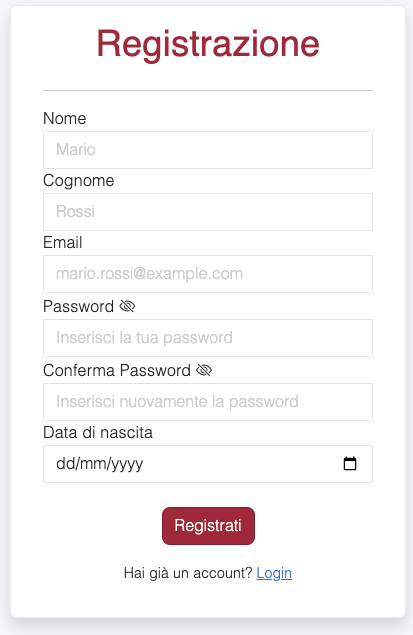
\includegraphics[width=0.5\textwidth]{registrazione}}\\
        \caption{\raggedleft Screenshot registrazione}
    \end{minipage}\hfill
    \begin{minipage}[c]{0.5\linewidth}
        \centering
        \fbox{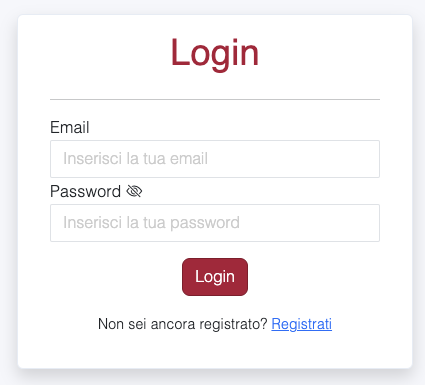
\includegraphics[width=0.7\textwidth]{login}}\\
        \caption{Screenshot login}
    \end{minipage}
\end{figure}

\subsection{Gestione dei progetti}
\subsubsection{Caricamento di un progetto} 
L'utente ha la possibilità di caricare un progetto allegando multipli file $.pdf$, per concludere l'operazione è necessario selezionare il tipo di progetto da un menù a tendina, inserire una breve descrizione e facoltativamente scrivere una nota a riguardo.
\subsubsection{Creazione degli stati per la valutazione}
I possibili stati di un progetto sono rimasti gli stessi descritti nel tema del progetto(Submitted, Require Changes, Approved, Not Approved), nella visualizzazione di un progetto l'utente può osservare ogni stato di tale progetto, al quale vengono affiancate 3 informazioni: i file allegati, le note del valutatore e la data.
\subsubsection{Valutazione dei progetti}
Un utente valutatore può cambiare lo stato dei progetti aggungendone uno nuovo, per farlo deve caricare uno o più file $.pdf$, così da poter mantenere il file originale e magari aggiungerne un altro con le eventuali correzioni, dopo aver caricato i file può selezionare il nuovo stato da un menù a tendina e aggiungere delle eventuali note, come indicato dal tema del progetto. 
\subsubsection{Chat}
In ogni progetto è presente una chat sulla quale possono scrivere il creatore del progetto e gli eventuali valutatori.
\begin{figure}[!h]
    \begin{minipage}[c]{0.5\linewidth}
        \centering
        \fbox{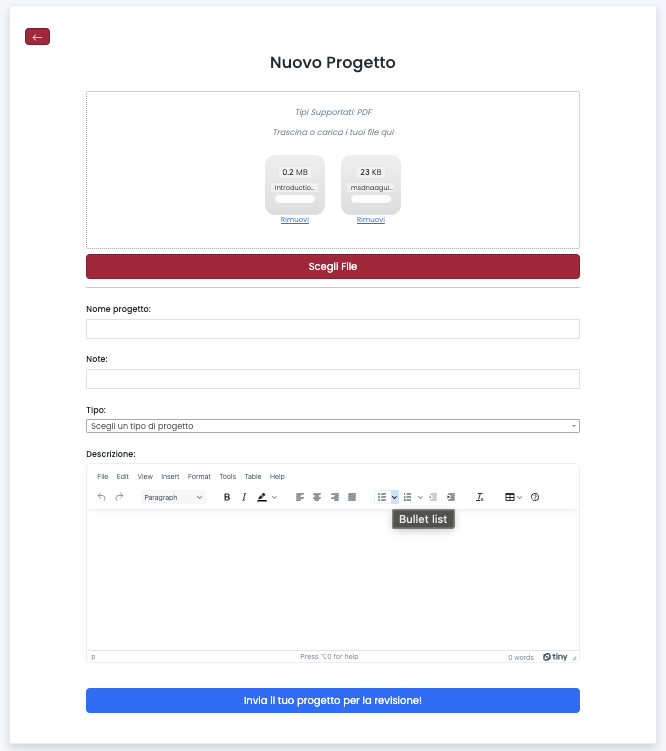
\includegraphics[width=0.7\textwidth]{nuovo}}\\
    \end{minipage}\hfill
    \begin{minipage}[c]{0.5\linewidth}
        \centering
        \fbox{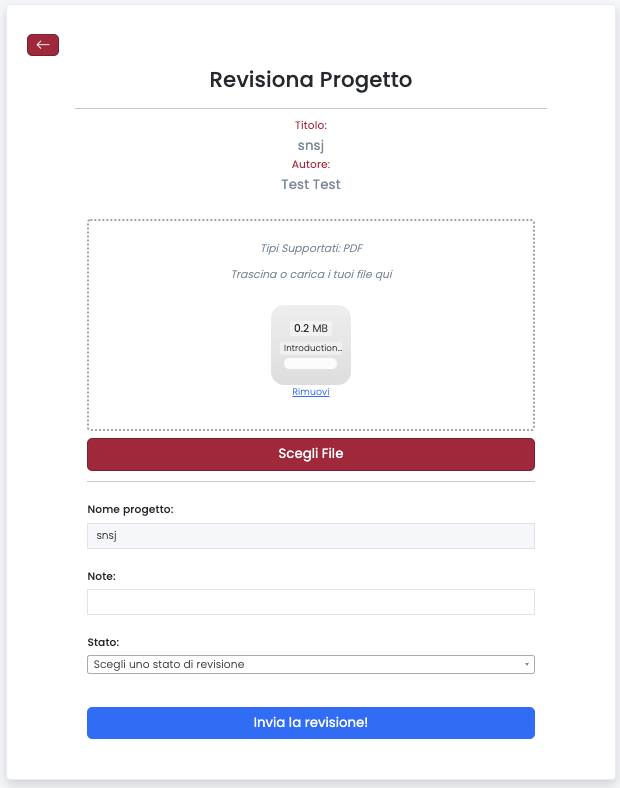
\includegraphics[width=0.7\textwidth]{valuta}}\\
    \end{minipage}
    \caption{Pagine per la creazione e la valutazione di un progetto}
\end{figure}

\begin{figure}[!h]
    \begin{minipage}[c]{0.5\linewidth}
        \centering
        \fbox{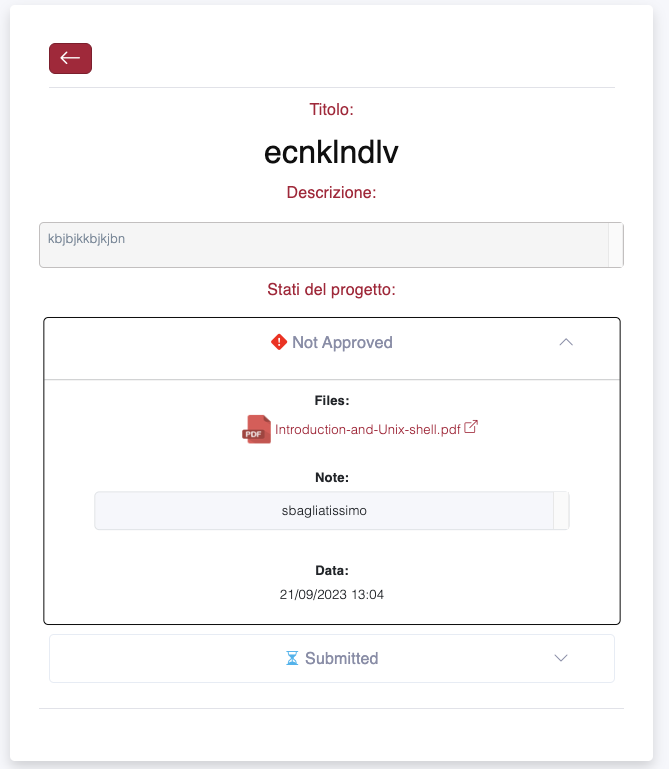
\includegraphics[width=0.7\textwidth]{stati}}\\
        \caption{Esempio di visualizzazione degli stati di un progetto}
    \end{minipage}\hfill
    \begin{minipage}[c]{0.5\linewidth}
        \centering
        \fbox{
\includegraphics[width=0.7\textwidth]{chat}}\\
        \caption{Chat di un progetto}
    \end{minipage}
\end{figure}


\subsection{Amministrazione}
\subsubsection{Ruoli}
L'assegnazione dei privilegi agli utenti dell'applicazione si basa su 3 ruoli: 
\begin{itemize}
    \item Researcher: è il ruolo con meno privilegi, può solo creare i propri progetti senza valutarne altri;
    \item Reviewer: è un Researcher che ha anche la possibilità di valutare i progetti degli altri utenti;
    \item Admin: può accedere alla Admin Dashboard e può anche valutare i progetti, questo ruolo viene assegnato dall'amministratore di sistema.
\end{itemize}
\subsubsection{Admin Dashboard}
Questa pagina consiste in una tabella interattiva con la quale l'utente admin può avere accesso ai dati anagrafici dei singoli utenti, modificarne il ruolo ed eventualmente rimuovere gli utenti dal sistema.
\begin{figure}[!h] 
    \centering
    \fbox{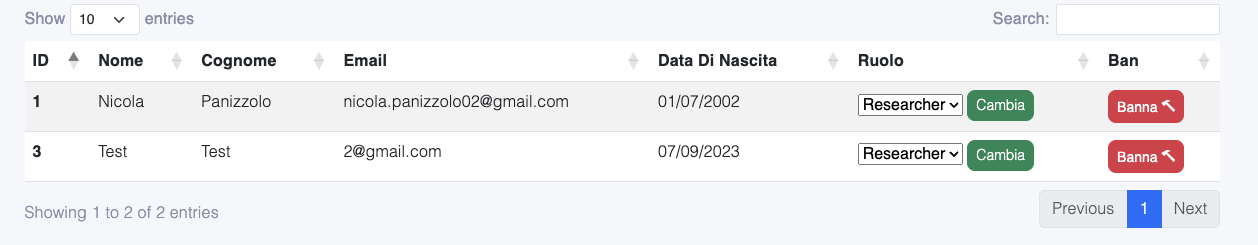
\includegraphics[width=0.9\textwidth]{admin}}\\
    \caption{Admin Dashboard}
\end{figure}

\section{Progettazione concettuale e logica della base di dati}

\section{Query principali}
\subsection{Metodologia}
Nel corso del nostro progetto, abbiamo scelto di utilizzare query molto semplici per interagire con il database. Questa scelta è stata guidata da due considerazioni principali.
\subsubsection{Nessuna Necessità di Richieste Particolari al Database}
Inizialmente, abbiamo valutato le nostre esigenze di accesso ai dati e abbiamo constatato che non vi era alcuna necessità di richieste particolari o complesse. Le informazioni di cui avevamo bisogno potevano essere recuperate in modo efficace attraverso query dirette e semplici. L'assenza di complessità nelle nostre richieste ha reso inutile l'uso di query più intricate.
\subsubsection{Struttura Ottimale del Database}
Un elemento chiave che ha influenzato la nostra scelta è stata l'ottima struttura del database. Le tabelle erano organizzate in modo chiaro e logico, con attributi ben definiti e relazioni ben gestite tra di loro. Questa struttura ha semplificato notevolmente l'interrogazione del database.


\subsection{Discussione}
Grazie all'adozione di query semplici, siamo stati in grado di ottenere risultati soddisfacenti nel nostro progetto. La struttura ben progettata delle tabelle del database è stata fondamentale in questo processo. 
Inoltre l'astrazione delle tabelle tramite i Model di Flask ha permesso di ridurre l'utilizzo dei join solo nel momento in cui strettamente necessario.
Di seguito, discutiamo alcune delle principali ragioni per cui abbiamo adottato questo approccio.
\subsubsection{Riduzione del Carico di Lavoro del Database}
L'uso di query semplici ha comportato un carico di lavoro minore sul database, riducendo il tempo di esecuzione delle operazioni, in quanto vengono sfruttati gli indici generati tramite le foreign keys.
\subsubsection{Facilità di Manutenzione}
La gestione di query semplici è stata vantaggiosa anche dal punto di vista della manutenzione. Le query erano facilmente comprensibili e modificabili, semplificando il processo di adattamento alle nuove esigenze del progetto.


\subsection{Query Principali}
\subsubsection{Creazione di un progetto}
La creazione di un progetto risulta essere una sequenza di query che vanno ad  effettuare l'insert in più tabelle.\\
\begin{enumerate}
    \item Utilizziamo la query seguente per produrre il menù a tendina dove l'utente può selezionare il tipo del progetto che sta andando a creare.
    \begin{lstlisting}
    SELECT id, name FROM types
    \end{lstlisting}
    Con la prossima query avviene l'effettiva creazione del progetto.
    \item 
    \begin{lstlisting}
    INSERT INTO projects( id_user, id_type, name, description) 
            VALUES (1,1, 'TEST', 'TEXT')
    \end{lstlisting}
    Per ottenere l'id\_user abbiamo utilizzato l'oggetto current\_user della classe flask\_login istanziato sulla base del risultato della query di login:
    \begin{lstlisting}
    SELECT * FROM users WHERE email='test@test.it'
    \end{lstlisting}
    \item Tramite flask abbiamo quindi la possibilità di ottenere l'id della row appena creata nella tabella projects.
    \item Otteniamo l'id stato “Submitted” tramite una query (ci servirà come valore di default).
    \begin{lstlisting}
    SELECT id FROM states WHERE name='Submitted'
    \end{lstlisting}
    \item Andiamo a creare lo stato (history) per questo nuovo progetto. Ci permetterà di avere uno storico di tutti gli stati del progetto.
    \begin{lstlisting}
    INSERT INTO project_history(id_project, id_state, id_user_reviewer) 
           VALUES (1,2,1)
    \end{lstlisting}
    \item Tramite flask abbiamo quindi la possibilità di ottenere l'id della row appena creata nella tabella projects\_history.
    \item Andiamo infine a definire il path di caricamento dei file per questo progetto in questo preciso stato.
    \begin{lstlisting}
    INSERT INTO project_files(path, id_project_history) VALUES 
        ('/app/db_files/1/1/1/TEST1.pdf',1),
        ('/app/db_files/1/1/1/TEST2.pdf',1),
        ('/app/db_files/1/1/1/TEST3.pdf',1)
    \end{lstlisting}
\end{enumerate}

\subsubsection{Elenco dei progetti da valutare}
Abbiamo avuto l'esigenza di dover mostrare ai reviewer solo i progetti che non sono stati chiusi affinché possano avere la possibilità di valutarli.
\begin{enumerate}
    \item  
    \begin{lstlisting}
    SELECT * FROM users WHERE id=1 AND id_role IN 
        (SELECT id FROM roles WHERE is_reviewer=TRUE)
    \end{lstlisting} 
    Se questa query (dove l'id corrisponde all'id dell'utente che ha effettuato il login) non ritorna alcuna riga blocchiamo l'accesso alla pagina in quanto l'utente non è autorizzato
    \item 
    \begin{lstlisting}
    SELECT *
    FROM projects
    WHERE id IN 
       (SELECT id_project
        FROM project_history
        WHERE id IN 
           (SELECT MAX(id)
            FROM project_history
            WHERE id_project NOT IN
                (SELECT id FROM projects WHERE id_user = 1)
            GROUP BY id_project)
        AND id_state IN 
           (SELECT id 
            FROM states
            WHERE is_closed = FALSE))    
    \end{lstlisting}
    Questa query ci permette di avere l'elenco di tutti i progetti, senza duplicati, che non sono stati creati dall'utente loggato (non vogliamo che un reviewer si possa approvare un progetto in modo autonomo) e che possiedono come ultimo stato attribuito (history) uno stato con flag “non chiuso”. 
    \item Andiamo quindi a prendere i tipi di progetto disponibili nel software, questo permetterà al backend in python di raggruppare gli oggetti Project in sezioni del dizionario Types divise per Project.id\_type ai fini una stampa ordinata per tipo:
    \begin{lstlisting}
    SELECT id, name FROM types
    \end{lstlisting}
\end{enumerate}


\section{Principali scelte progettuali}
\subsection{Trigger}
Il trigger \textbf{is\_reviewer\_trigger} implementa un rigoroso controllo di validazione per garantire che gli utenti designati come revisori siano effettivamente qualificati come tali prima di consentire loro di apportare inserimenti o aggiornamenti alla tabella project\_history. Inoltre estende la possibilità di inserimento per un dato progetto agli utenti che non sono qualificati come revisori ma sono autori dello stesso. 
Questa funzione rappresenta una soluzione efficace per garantire l'integrità dei dati e la conformità alle regole imposte dal sistema di valutazione.
\begin{lstlisting}
CREATE OR REPLACE FUNCTION is_reviewer()
RETURNS TRIGGER AS
$$
BEGIN
IF NEW.id_user_reviewer IS NOT NULL THEN
IF (NEW.id_user_reviewer NOT IN
(SELECT u.id
FROM users u JOIN roles r ON u.id_role=r.id
WHERE r.is_reviewer AND u.id=NEW.id_user_reviewer) AND
(NEW.id_user_reviewer != (SELECT id_user FROM projects WHERE id=NEW.id_project))
) THEN
RETURN NULL;
END IF;
END IF;
RETURN NEW;
END $$ LANGUAGE plpgsql;

CREATE OR REPLACE TRIGGER is_reviewer_trigger
BEFORE INSERT OR UPDATE ON project_history
FOR EACH ROW EXECUTE FUNCTION is_reviewer()
\end{lstlisting}
\subsection{Sicurezza}
È stata adottata una soluzione avanzata basata su Docker per garantire un elevato grado di isolamento e controllo dell'accesso al database e ogni dato viene analizzato prima di essere inserito nella base di dati.
In particolare il progetto, sotto il punto di vista della sicurezza, tocca i seguenti punti:
\begin{itemize}
    \item Container Docker Isolato: Per garantire un ambiente altamente sicuro, è stato creato un contenitore Docker isolato dal resto della rete. L'isolamento è fondamentale per proteggere il database da accessi non autorizzati in particolare: 
    \begin{itemize}
        \item Accesso Limitato agli Utenti: Solo due utenti hanno accesso a questo database, il superutente (root) e un utente specifico denominato "progetto";
        \item Network Isolata: Il container Docker è configurato in modo da essere completamente isolato dalla rete esterna. Questo significa che il database non è accessibile dalla rete pubblica o da altre risorse di rete, garantendo una protezione aggiuntiva contro attacchi esterni;
        \item Controllo Preciso dell'Accesso: limitare l'accesso al database solo al container Python impedisce ad altri servizi o applicazioni non autorizzati di interagire direttamente con il database.
    \end{itemize}
    \item Sanitizzazione delle Query: tutte le query eseguite nel database sono sanificate attraverso SQLAlchemy ORM:
    \begin{itemize}
        \item Prevenzione degli Attacchi SQL Injection: L'ORM SQLAlchemy è progettato per prevenire gli attacchi di SQL injection, in quanto sanitizza automaticamente le query, impedendo l'inserimento di codice SQL dannoso;
        \item Prevenzione degli Attacchi XSS: dove l'ORM non può arrivare siamo intervenuti manualmente a sanificare i dati in modo che i testi stampati nel DOM (descrizione dei progetti, note e messaggi della chat) fossero sanificati anche da iniezioni di codice JavaScript.
    \end{itemize}
\end{itemize}

\subsection{Politiche di autorizzazione}
La tabella "Roles" è progettata per contenere informazioni sulle tipologie di ruoli assegnabili agli utenti del sistema. Ogni utente è associato a un ruolo specifico attraverso un campo "id\_role". La gestione delle politiche di autorizzazione per la valutazione dei progetti è implementata attraverso la tabella "Roles" in questo modo:
\begin{itemize}
    \item Flag per Valutazione dei Progetti: all'interno della tabella "Roles", è presente un flag che indica se gli utenti con quel ruolo specifico hanno il permesso di valutare i progetti;
    \item Ruolo dell'Amministratore(id\_role=1): L'utente con "id\_role=1", ovvero l'amministratore, è l'unico che può:
    \begin{itemize}
        \item Cambiare i ruoli degli altri utenti: questo privilegio consente all'amministratore di assegnare o revocare il diritto di valutare i progetti ad altri utenti;
        \item Bannare: in caso di comportamenti ritenuti non corretti ha la possibilità di bloccare l'accesso agli utenti incriminati.
    \end{itemize}
    \item Privilegi Amministrativi: La gestione dei privilegi amministrativi è stata configurata in modo da impedire che un utente possa promuovere(se stesso o altri) a ruolo di amministratore. Per farlo è necessario un intervento diretto da parte degli sviluppatori del sistema all'interno del database, previa esplicita richiesta.
\end{itemize}

\subsection{Performance}
Nella progettazione e nell'utilizzo del database, abbiamo adottato una strategia di ottimizzazione basata sull'utilizzo di indici generati dalle foreign key delle tabelle del database e sfruttato il "lazy loading" implicito offerto da SQLAlchemy per massimizzare le performance.\\\\In modo specifico, gli indici Foreign Key consentono quanto segue:
\begin{itemize}
    \item Join Efficienti: Quando si eseguono operazioni di join tra tabelle che condividono chiavi esterne, la presenza di indici FK riduce notevolmente il tempo necessario per effettuare join;
    \item Mantenimento dell'Integrità dei Dati: Gli indici FK impediscono l'inserimento di dati non validi nelle tabelle. Ciò contribuisce a garantire che i dati siano coesi e che rispettino le relazioni previste.
\end{itemize}
Mentre il Lazy Loading Implicito di SQLAlchemy offre i seguenti vantaggi:
\begin{itemize}
    \item Accesso On-Demand: Quando si accede a un oggetto collegato tramite una relazione, SQLAlchemy carica solo quei dati dal database che sono necessari in quel momento, evitando il caricamento eccessivo di dati inutilizzati;
    \item Riduzione del Carico di Lavoro del Database: L'uso del lazy loading impedisce al database di eseguire query pesanti in modo prematuro, contribuendo a ridurre il carico di lavoro del database e a migliorare le prestazioni complessive del sistema.
\end{itemize}

\section{Ulteriori informazioni}
Per la realizzazione dell'applicazione sono state utilizzate diverse librerie e framework, alcuni per lo sviluppo del backend e alcuni di frontend.
\subsection{Backend}
\subsubsection{Flask}
Flask è un micro-framework web leggero e flessibile per la creazione di applicazioni web in Python. È progettato per essere semplice da imparare e utilizzare, consentendo agli sviluppatori di creare rapidamente applicazioni web con un minimo sforzo. Flask offre funzionalità di base per la gestione delle richieste HTTP, la creazione di route, la gestione dei template HTML e l'integrazione di database, ma è altamente estendibile grazie all'ampia disponibilità di estensioni e plug-in. Flask è particolarmente adatto per progetti più piccoli o applicazioni web leggere, ed è ampiamente utilizzato per la creazione di servizi web, API e prototipi.
\subsubsection{Flask Login}
Flask-Login è un'estensione per il framework web Flask in Python che semplifica l'implementazione dell'autenticazione utente in un'applicazione web. Questa estensione fornisce funzionalità per la gestione delle sessioni utente, la verifica delle credenziali, il riconoscimento degli utenti autenticati e la protezione delle route o delle risorse dell'applicazione che richiedono l'autenticazione.
\subsubsection{SQLAlchemy}
SQLAlchemy è una libreria Python molto popolare per la gestione delle operazioni di accesso e manipolazione dei database relazionali. Essa fornisce un'interfaccia ad alto livello per comunicare con database SQL, rendendo più semplice e astratta l'interazione con i database da parte degli sviluppatori.

\subsection{Frontend}
\subsubsection{Bootstrap 5}
Bootstrap 5 è una delle versioni più recenti del framework di front-end open-source Bootstrap, utilizzato per la progettazione e lo sviluppo di siti web e applicazioni web. In sintesi Bootstrap 5 fornisce un set di strumenti e componenti per la creazione di siti web e applicazioni web moderni, reattivi e personalizzabili. Le sue caratteristiche di personalizzazione, design responsive e utilizzo semplice lo hanno reso la chiave per lo sviluppo front-end dell'applicazione.
\subsubsection{Jquery}
Jquery è una libreria JavaScript open-source ampiamente utilizzata per semplificare la manipolazione del DOM (Document Object Model) e l'interazione con gli elementi HTML all'interno di pagine web, nel progetto è stata fondamentale per semplificare lo sviluppo di alcune funzioni secondarie.
\subsubsection{Dropzone}
Nelle pagine dove gli utenti caricano i progetti viene viene utilizzata Dropzone.js: è una libreria JavaScript open-source che semplifica l'implementazione del caricamento di file da parte degli utenti in un'applicazione web.
\subsubsection{TinyMCE}
TinyMCE è un editor di testo WYSIWYG (What You See Is What You Get) open-source ampiamente utilizzato per l'integrazione in applicazioni web e siti web. Il nome "TinyMCE" è l'acronimo di "Tiny Moxiecode Content Editor", è utilizzato da qualsiasi sito web o applicazione che richiede un editor di testo WYSIWYG per consentire agli utenti di creare e modificare contenuti in modo intuitivo, nel nostro caso viene utilizzato per la descrizione dei progetti.
\subsubsection{Socket.IO}
Socket.IO è una libreria JavaScript open-source che consente la comunicazione bidirezionale in tempo reale tra un server web e un client web. È spesso utilizzato per implementare applicazioni web interattive, chat in tempo reale, giochi online e altre applicazioni che richiedono una comunicazione istantanea tra il server e il client. Nel nostro scenario, Socket.IO offre un modo efficiente per consentire la comunicazione in tempo reale tra i partecipanti ai progetti di ricerca all'interno dell'applicazione. Consentendo ai proprietari dei progetti e ai valutatori di scambiare informazioni istantaneamente, migliora l'efficienza e la collaborazione all'interno del sistema di valutazione dei progetti.
\begin{figure}[H]
    \begin{minipage}[c]{0.5\linewidth}
        \centering
        \fbox{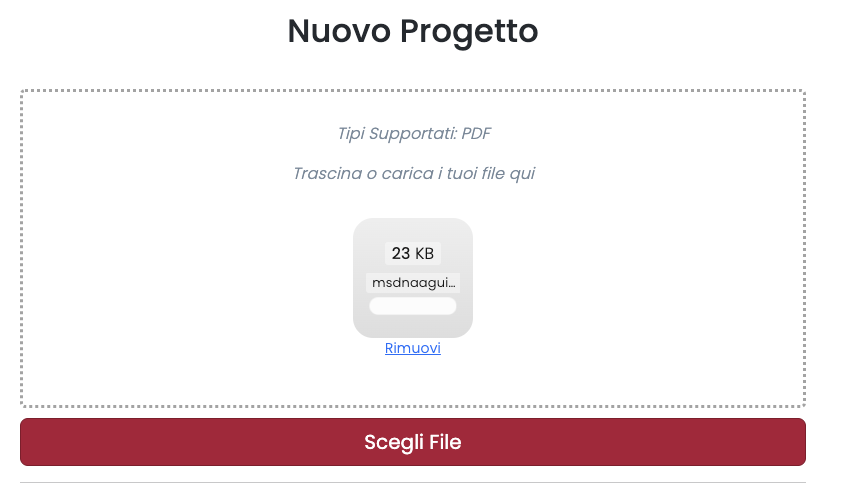
\includegraphics[width=0.9\textwidth]{dropzone}}\\
        \caption{Dropzone per il caricamento dei progetti}
    \end{minipage}\hfill
    \begin{minipage}[c]{0.5\linewidth}
        \centering
        \fbox{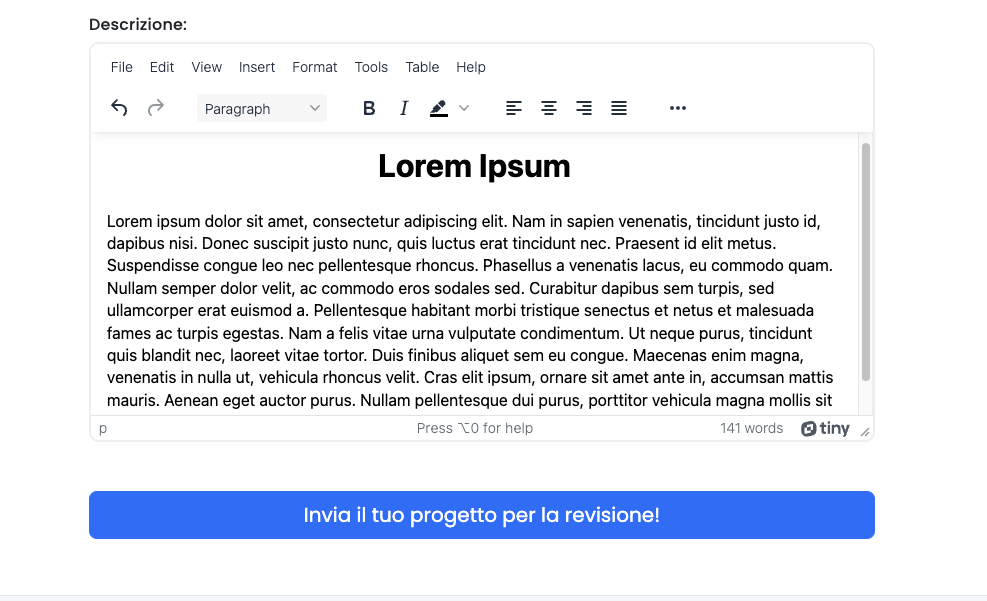
\includegraphics[width=0.9\textwidth]{tiny}}\\
        \caption{TinyMCE per la descrizione dei progetti}
    \end{minipage}

\end{figure}

\section{Contributo al progetto}

\end{document}